\documentclass[letterpaper, 10 pt, conference]{sty/ieeeconf}

\IEEEoverridecommandlockouts

\overrideIEEEmargins

\usepackage{graphics}
\usepackage{epsfig}
\usepackage{amsmath}
\usepackage{amssymb}
\usepackage{txfonts}
\usepackage{tikz}
\usepackage[T1]{fontenc}

\DeclareMathOperator*{\argmax}{arg\,max}
\DeclareMathOperator*{\argmin}{arg\,min}

\begin{document}

\title{\LARGE \bf
Curbs Detection for a Pedestrian Robot
}

\author{
\authorblockN{
J\'{e}r\^{o}me Maye,
Ralf Kaestner,
and Roland Siegwart}
\authorblockA{
Autonomous Systems Lab, ETH Zurich, Switzerland\\
email: \{jerome.maye, ralf.kaestner, roland.siegwart\}@mavt.ethz.ch}
}

\maketitle

\begin{abstract}
This paper presents a novel ...

\end{abstract}

\section{Introduction}
Urban areas are highly complex environments which introduce numerous challenges
to autonomous service robots. In particular, for a safe and reliable navigation,
a robot should be able to accurately detect curbs. Curbs usually appear at the
borders between streets and sidewalks. The knowledge of curb positions and
characteristics can beneficially enhance metric maps with traversability
information relevant to navigation. For instance, depending on its physical
capabilities, a robotic platform could only drive harmlessly over curbs of a
given height when crossing a street.

Amongst the difficulties related to this task, curbs might exhibit various
curvatures and heights, and be perceived from different viewpoints. In contrast
to autonomous cars, pedestrian robots can indeed make few assumptions about
the structure of the environment. Furthermore, the sensing device noise model
should be introduced to distinguish between real curbs and measurement noise.
Ideally, the algorithm should run on-line and in real-time.

In this paper, we devise an unsupervised method to curb detection that covers
most of the aforementioned requirements. Our approach attempts to construct a
piecewise planar model of the environment and determines curbs at plane segment
boundaries. Initially, we sense the environment with a nodding laser
range-finder and project the 3D measurements into an efficient Digital Elevation
Map (DEM). Each cell of the DEM maintains an error model that is propagated
throughout the entire algorithm. Plane segments are further estimated with a
mixture of linear regression model. Here, we propose an original formulation of
the standard Expectation-Maximization (EM) algorithm for mixture models.
Specifically, in the E-step, the responsibilities are computed with a
Conditional Random Field (CRF) that introduces dependencies between the
covariates of the mixture model. A graph-based segmentation of the DEM provides
an estimate of the number of planes and initial parameters for the EM.
Sequential and fast estimations of DEM patches in the surrounding of the sensor
while the robot drives ensure on-line operation. Fig.~\ref{fig:intro} shows a
typical output of our algorithm with the curb points reprojected on the original
data.

\begin{figure}[t]
\centering
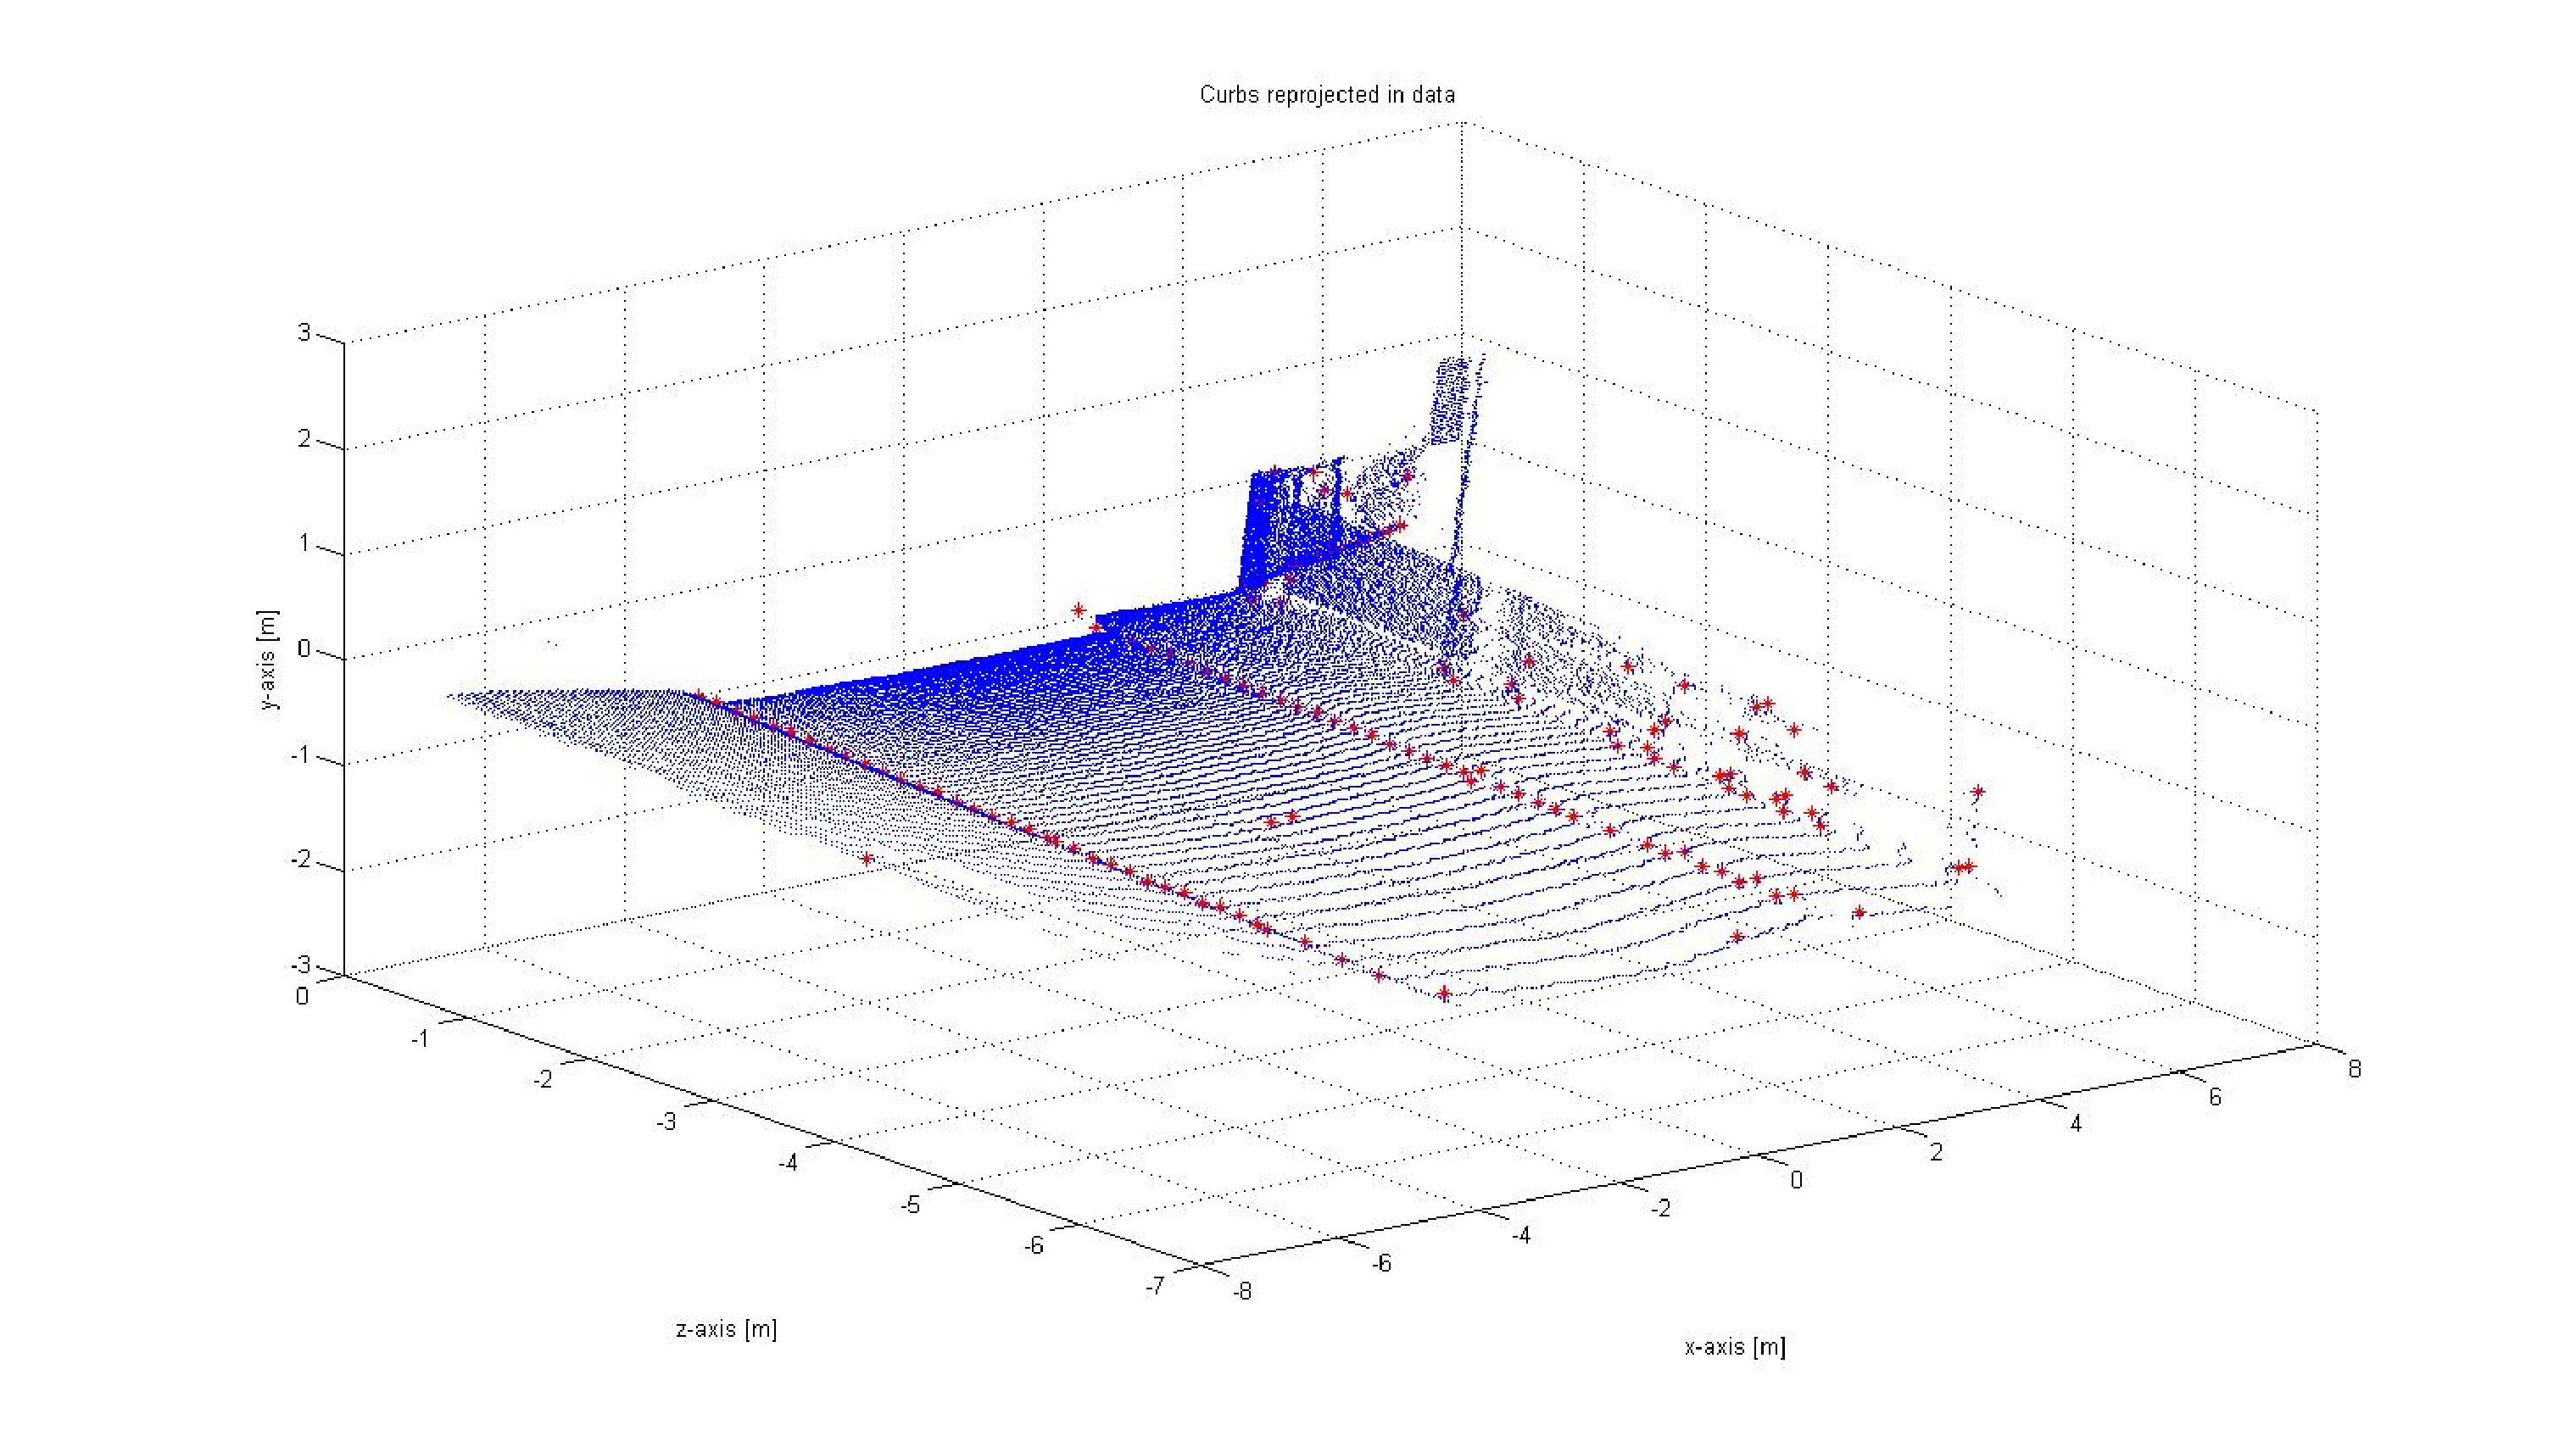
\includegraphics[width=\columnwidth]{fig/intro.eps}
\caption{Exemplary output of our curb detection algorithm. Curb points
(red stars) are reprojected into the original point cloud.}
\label{fig:intro}
\end{figure}

Clearly, the main contribution of the paper is its strict probabilistic
interpretation from the sensing process to the final plane estimation and
segmentation. Moreover, our method is view-independent and requires no
particular prior knowledge about the environment. The set of free parameters
is solely related to the sensor characteristics and involves no hand-tuning.
Finally, a direct implementation of the algorithm from the paper should be
straightforward.

The remainder of the paper is structured as follows. Section~\ref{sec:related}
summarizes the previous works related to ours. Section~\ref{sec:model}
introduces our statistical models and derives the related inference methods.
Section~\ref{sec:implementation} is concerned with implementation and
algorithmic details. Section~\ref{sec:exp} demonstrates the validity of the
method through extensive qualitative and quantitative analysis.
Section~\ref{sec:conc} outlines our conclusions and provides some insights for
future work.


\section{Related Work\label{sec:related}}
The problem of curb or \emph{step} detection has mainly been studied in the
context of Intelligent Transportation Systems (ITS), covering an extensive set
of sensing modalities and algorithms. In ITS, one might assume a typical
experimental setting where a car drives on a street and curbs are situated on
the left and right side of the vehicle. Therefore, most of these approaches
are inappropriate as such for a pedestrian robot navigating in cities. In this
situation, curbs will indeed appear under multiple viewpoints. We hence review
the main influential contributions to the field and relate them to our method.

In~\cite{oniga10polynomial}, Oniga \emph{et al.} employ a dense stereo-vision
system to capture a 3D point cloud, which is further transformed into a Digital
Elevation Map (DEM). Curbs are represented as third-order polynomials. Candidate
curb points are extracted with a Canny edge detector. A RANdom SAmple Consensus
(RANSAC) polynomial fitting is then applied to perform outlier rejection and
find the polynomial coefficients. The location of the curbs and their heights
are finally obtained with some further refinement steps. In comparison to this
method, we use the same measurement representation (DEM). However, we draw a
clear and sound probabilistic model from the sensing device to the curb
detection and limit the number of hand-tuned parameters.

Closer to our approach, Siegemund \emph{et al.}~\cite{siegemund10curb} proposed
a promising method that extracts curbs from dense stereo-vision data. We
actually take inspiration on their ideas and solve their major drawbacks. In
this paper, as mentioned above, they assume a strict environment model and they
lack a unified probabilistic model. Moreover, their curb models can only
represent a limited set of curbs. For instance, they cannot model T
junctions or roundabouts.

In~\cite{shin10drivable}, Shin \emph{et al.} use a similar setup as ours, i.e.,
a mobile robot equipped with a laser range-finder. They however stick to a
restricted environment model and their tilted laser only provides a single laser
line. Their algorithm is mostly engineered to fit their particular application
and setup, and again does not build on sound probabilistic model.

An alternative application of step detection is presented
in~\cite{pradeep08piece}. In this paper, Pradeep \emph{et al.} aim at mobility
aids for visually impaired people, as a complement to the white cane or the dog.
This naturally imposes restrictions in the sensing device, in this case a
wearable and cheap stereo camera. Their curb detection algorithm is based on the
same motivation as ours, i.e., building a piecewise planar model of the scene.
In their implementation, point-wise normal vectors are firstly estimated with
Principal Component Analysis on a local neighborhood and RANSAC for outlier
rejection. Tensor voting is then applied for finding globally consistent plane
normals and a final clustering step extracts the plane segments. Although it
solves many of the above issues, this method might also suffer from the lack of
any underlying probabilistic models.

In~\cite{yuan05dynamic}, Yuan and Manduchi also developed an algorithm for
visually impaired people, working with a custom sensing device called
a "Virtual White Cane". Their method uses a Jump-Markov Process to detect
geometric singularities in the range measurements. Despite its statistical
foundations, it will not generalize well to our application requirements and
provide a plane estimation.


\section{Model\label{sec:model}}
\subsection{Measurements Representation}
Scan measurements $\mathbf{s}_i=[r_i,\theta_i,\psi_i]^\text{T}$ are transformed
into their corresponding Cartesian 3D coordinates $\mathbf{p}_i=[x_i,y_i,z_i]
^\text{T}$, where $r_i$ is a range measurement, $\theta_i$ a pitch angle, and
$\psi_i$ a bearing angle. From a complete laser sweep, we obtain a point cloud
representation $\mathcal{P}=\{\mathbf{p}_1,\mathbf{p}_2,\dots,\mathbf{p}_N\}$.
$\mathcal{P}$ is finally projected onto a 2D grid $\mathcal{G}=\{\mathcal{C}_1,
\mathcal{C}_2,\dots,\mathcal{C}_M\}$, with cells $\mathcal{C}_i=
\{\mathbf{ul}_i,\mathbf{lr}_i,\mathbf{c}_i,h_i,l_i,\mathcal{I}_i\}$, where
$\mathbf{ul}_i$ and $\mathbf{lr}_i$ are the upper left and lower right 2D
coordinates of the cell, $\mathbf{c}_i$ the center of the cell, $h_i$ the height
of the cell such that $h_i\propto\mathcal{N}(\mu_i,\sigma_i)=p(h_i\mid\mu_i,
\sigma_i,\mathcal{I}_i)$, $l_i\in\{1,\dots,M\}$ a discrete label for the cell,
and $\mathcal{I}_i=\{\mathbf{p}_j\mid\mathbf{p}_j\in\mathcal{P},
\mathbf{p}_{j_x}>\mathbf{ul}_{i_x},\mathbf{p}_{j_y}>\mathbf{ul}_{i_y}
,\mathbf{p}_{j_x}<\mathbf{lr}_{i_x},\mathbf{p}_{j_y}<\mathbf{lr}_{i_y}
,\mathbf{p}_{j_z}<\theta_U,\mathbf{p}_{j_z}>\theta_L\}$. $\theta_U$
and $\theta_L$ define upper and lower bounds for the height values.

The grid $\mathcal{G}$ will also be referred to as a Digital Elevation Map (DEM)
in the rest of the paper. The choice of a DEM representation is mainly guided by
the final outcome of the algorithm, i.e. a traversability map for the planning
process. It is also convenient for defining Regions of Interest (ROI) in
$\mathcal{P}$ and for simplifying the subsequent computations. We could also
have resorted to a polar grid representation, so as to have a finer resolution
close to the sensor (THIS IS STILL OPEN AND NEED FURTHER EXPLANATIONS). Whenever
the number of points in a cell $\mathcal{C}_i$ is below a threshold, i.e.
$|\mathcal{I}_i|<\theta_P$, it is flagged as invalid.

REMARKS:
\begin{itemize}
\item EXPLAIN HOW WE CAN GO FROM THE PUSH-BROOM LASER DATA TO THE DEM
\item EXPLAIN WHAT HEIGHT $h_i$ IS FINALLY TAKEN
\end{itemize}

\subsection{Environment Model and Inference Task}
We assume a piecewise planar environment, i.e., the observed scene is composed
of a set of plane segments $\mathcal{S}_1,\mathcal{S}_2,\dots,\mathcal{S}_M$, with
$\mathcal{S}_i=\{\mathcal{C}_j\mid h_j=\mathbf{w}_i^\text{T}\boldsymbol{\phi}
(\mathbf{c}_{j})\}$, $\mathbf{w}_i=[w_0^{(i)}, w_1^{(i)}, w_2^{(i)}]^\text{T}$,
and $\boldsymbol{\phi}(\mathbf{c}_{j})=[1,\mathbf{c}_j]^\text{T}$.

Boundaries between plane segments define local heights discontinuities that we
shall term \emph{curbs} from now on. The major inference task therefore boils
down to discovering those plane segments. To this end, we follow a probabilistic
and iterative approach.


\section{Initial Labeling\label{sec:initial}}
Our algorithm needs an initial rough estimate of the plane segments. This
initial estimate consists in labeling the DEM cells that belong to the same
plane segments. More formally, we refine our definition of plane segments to
$\mathcal{S}_i=\{\mathcal{C}_j\mid l_j=i\}$.

We use the graph-based algorithm from Felzenzswalb and
Huttenlocher~\cite{felzenszwalb04efficient}. Although this method was originally
designed for image segmentation, we can tune it for our purposes, image regions
corresponding to plane segments. We define an undirected graph
$\mathcal{G}=\{\mathcal{V},\mathcal{E}\}$, with vertices $v_i\in\mathcal{V}$ to
be segmented and edges $(v_i,v_j)\in\mathcal{E}$ for neighboring vertices. Each
edge has a weight $w((v_i,v_j))$ proportional to the dissimilarity between $v_i$
and $v_j$. In our particular setting, each grid cell $\mathcal{C}_i$ is aligned
with a vertex $v_i$ and each vertex has a 4-connected neighborhood. The goal of
the algorithm is to find a partition of $\mathcal{V}$ into components
$\mathcal{C}$ that correspond to the connected components of a graph
$\mathcal{G}'=\{\mathcal{V},\mathcal{E}'\}$, with
$\mathcal{E}'\subseteq\mathcal{E}$. We are interested in the partition such that
vertices in a component have a high similarity and vertices in different
components a low similarity. Therefore, edges between vertices in the same
component should have a low weight and edges between vertices in different
components a high weight. We define the weight function as the symmetric
Kullback-Leibler divergence between two cells, i.e.,
$w((v_i,v_j))=D_{KL}(h_i\mid\mid h_j)+D_{KL}(h_j\mid\mid h_i)$. For normal
distributions, the Kullback-Leibler divergence integrates analytically to
$D_{KL}(h_i\mid\mid h_j)=\frac{(\mu_i-\mu_j)^2}{2\sigma_j^2}+\frac{1}{2}
(\frac{\sigma_i^2}{\sigma_j^2}-1-\ln\frac{\sigma_i^2}{\sigma_j^2})$. The
algorithm starts with all vertices belonging to a different component. It then
iterates by merging components based on the comparison predicate

\begin{equation}
\label{eqn:comp_pred}
D(C_1,C_2) = \left\{
\begin{array}{l l}
\text{true} & \quad \text{if $Dif(C_1,C_2)>MInt(C_1,C_2)$ }\\
\text{false} & \quad \text{otherwise},
\end{array} \right.
\end{equation}

where $Dif(C_1,C_2)=\min w((v_i,v_j))$, $Int(C)=\max w(e)$,
$MInt(C_1,C_2)=\min(Int(C_1)+\tau(C_1),Int(C_2)+\tau(C_2))$ the minimum internal
difference, and $\tau(C)=k/|C|$. Two components should be disconnected if the
difference between them is large compared to the internal difference within at
least one of the components. $k$ is a scale parameter that controls the
preference for larger components. The algorithm runs in $O(m\log(m))$, where
$m$ is the number of edges in the graph and it is guaranteed to produce a
segmentation which is neither too fine nor too coarse.

The resulting segmentation defines a probability distribution $p(l_i^{(0)})$ for
each cell, with the domain of $l_i$ being the number of components. This initial
distribution is expressed as

\begin{equation}
\label{eqn:comp_pred}
p(l_i^{(0)}=j) = \left\{
\begin{array}{l l}
1 & \quad \text{if $C_i$ belongs to component $j$}\\
0 & \quad \text{otherwise}.
\end{array} \right.
\end{equation}


\section{Planes Estimation\label{sec:plane}}
Given a labeling of the DEM cells belonging to the same plane segments, we show
here how we can get an estimate of the plane parameters using a Bayesian linear
regression framework.

At time step $t$ of the algorithm, we assume the following model for the plane
segment $j$

\begin{equation}
\label{eqn:regression1}
p(h_i\mid\mathbf{c}_i,\sigma^2_i,l_i,\mathbf{w}_j,\sigma^2_j)=\mathcal{N}(h_i|\mathbf{w}_j^\text{T}
\boldsymbol{\phi}(\mathbf{c}_i),\sigma^2_j).
\end{equation}

Since the $h_i$ are drawn independently, we can write the conditional likelihood

\begin{equation}
\label{eqn:regression2}
p(\mathbf{h}\mid\mathbf{C},\mathbf{w}_j,\sigma^2_j)=\prod_{i=1}^N\mathcal{N}(h_i|
\mathbf{w}_j^\text{T}\boldsymbol{\phi}(\mathbf{c}_i),\sigma^2_j),
\end{equation}

where $\mathbf{h}=[h_1,h_2,\dots,h_N]$ and $\mathbf{C}=[\mathbf{c_1},
\mathbf{c_2},\dots,\mathbf{c_N}]$.

We introduce a prior for the parameters to be estimated

\begin{equation}
\label{eqn:regression3}
p(\mathbf{w},\beta)=p(\beta)p(\mathbf{w}\mid\beta)
\end{equation}

where $p(\beta)$ is an inverse-gamma distribution and
$p(\mathbf{w}\mid\beta)$ a normal distribution.

The posterior distribution becomes

\begin{equation}
\label{eqn:regression4}
p(\mathbf{w}\mid\mathbf{h})=\mathcal{N}(\mathbf{w}\mid \mathbf{m}_N,
\mathbf{S}_N),
\end{equation}

where

\begin{eqnarray}
\label{eqn:regression5}
\mathbf{m}_N&=&\mathbf{S}_N(\mathbf{S}_0^{-1}\mathbf{m}_0+\beta
\boldsymbol{\Phi}^\text{T}\mathbf{h})\\\nonumber
\mathbf{S}_N^{-1}&=&\mathbf{S}_0^{-1}+\beta\boldsymbol{\Phi}^\text{T}\boldsymbol{\Phi}
\end{eqnarray}

and

\begin{equation}
\label{eqn:regression6}
\boldsymbol{\Phi}=
\left(
\begin{array}{cccc}
\phi_0(\mathbf{c}) & \phi_1(\mathbf{c}) & \cdots & \phi_{M-1}(\mathbf{c})\\
\phi_0(\mathbf{c}) & \phi_1(\mathbf{c}) & \cdots & \phi_{M-1}(\mathbf{c})\\
\cdots             & \cdots             & \ddots & \cdots\\
\phi_0(\mathbf{c}) & \phi_1(\mathbf{c}) & \cdots & \phi_{M-1}(\mathbf{c})\\
\end{array} \right)
\end{equation}


\section{Labeling with Conditional Random Field\label{sec:crf}}
Starting from the regression parameter set $\Theta$, we aim at computing the new
responsibilities $\gamma_{ik}$. In the classical mixture model framework, this
step is achieved by estimating

\begin{equation}
\label{eqn:responsibilities}
\gamma_{ik}\propto \pi_k\mathcal{N}(h_i\mid\mathbf{w}_k^\text{T}
\boldsymbol{\phi}(\mathbf{c}_i),\sigma^2_k).
\end{equation}

However, in our approach, we take the assumption that neighboring cells are more
likely to share the same label distribution, i.e., to be in the same plane
segment. A Conditional Random Field (CRF)~\cite{lafferty01conditional}
can advantageously propagate this information at a global scale on the entire
DEM and thus act as a \emph{smoother}. The initial labeling method from
Section~\ref{sec:initial}, due to its inherent local nature, might indeed result
in an over-segmented graph, that can be conveniently refined by the CRF.
Furthermore, a CRF provides the clear and sought probabilistic outcome in terms
of the distributions over $l_i$.

A CRF is a discriminative and undirected graphical model globally conditioned on
the observations. In our setting, we use the same graph structure
$\mathcal{G}=\{\mathcal{V},\mathcal{E}\}$ as in Section~\ref{sec:initial} and
the task of the CRF is to infer the label distributions $l_i$ for each node.

We want to express the conditional joint distribution of the CRF as

\begin{eqnarray}
\label{eqn:crf_joint}
p(\mathbf{l}\mid\mathbf{h},\Theta)\propto
\phantom{aaaaaaaaaaaaaaaaaaaaaaaaaaaaaaaaaa}\\ \nonumber
\exp\bigg(\sum_{v_i\in\mathcal{V}}
\varphi(h_i,l_i,\Theta)+\sum_{(v_i,v_j)\in\mathcal{E}}
\psi(h_i,h_j,l_i,l_j,\Theta)\bigg),
\end{eqnarray}

where $\mathbf{l}=[l_1,l_2,\dots,l_{M'}]^\text{T}$, and $\varphi=
\lambda\,f(h_i,l_i,\Theta)$ and $\psi=\mu\,g(h_i,h_j,l_i,l_j,\Theta)$ are the
\emph{node potential} and the \emph{edge potential}, respectively. The potential
functions are positively defined functions. Intuitively, the node potential
reflects the likelihood of $h_i$ being labeled $l_i$, and the edge potential the
joint likelihood of $h_i$ and $h_j$ being labeled $l_i$ and $l_j$. In the
original formulation of CRF, the MLE of the weights $\lambda$ and $\mu$ are
learned from training data. Since we apply the CRF in an unsupervised manner, we
fix these weights empirically.

According to the above suggestions, we define the feature function as

\begin{equation}
\label{eqn:feature_function}
f(h_i,l_i=k,\Theta)=\pi_k\mathcal{N}(h_i\mid\mathbf{w}_k^\text{T}
\boldsymbol{\phi}(\mathbf{c}_i), \sigma^2_{h_i} + \sigma^2_k).
\end{equation}

In Equ.~\eqref{eqn:feature_function}, we note that the CRF does not required a
normalized feature function. Moreover, by adding up the two variances, we have
inherently taken into account the measurement noise introduced by both error
models, namely the cell variance $\sigma^2_{h_i}$ and the regression variance
$\sigma^2_{k}$.

In analogy to the approach presented in~\cite{siegemund10curb}, we express the
inter-node dependencies by means of two symmetric sigmoid functions. Therefore,
we define the edge function as

\begin{eqnarray}
\label{eqn:edge_function}
g(h_i,h_j,l_i=k,l_j=l,\Theta)=\phantom{aaaaaaaaaaaaaaaaaaaaaaa}\\ \nonumber
\left\{
\begin{array}{l l}
1-(1+\exp(\sigma^2_{ij}-d_{ij}))^{-1} & \quad
\text{if $k=l$}\\
(1+\exp(\sigma^2_{ij}-d_{ij}))^{-1} & \quad
\text{otherwise},
\end{array} \right.
\end{eqnarray}

where $d_{ij}=|h_i-h_j|$ is the absolute height difference between the
neighboring cells $\mathcal{C}_i$ and $\mathcal{C}_j$. Additionally,
$\sigma^2_{ij}=\sigma^2_i+\sigma^2_j$ represents the sum of the involved
measurement variances. Hence, we again account for the errors in both cell
models $\sigma^2_i$ and $\sigma^2_j$.

Once the node and edge potential functions are defined, we can finally perform
inference on the CRF. In our configuration, \emph{Loopy} Belief
Propagation (LBP)~\cite{weiss00correctness} is an appropriate approach. LBP is
an approximate message-passing algorithm that computes the marginal distribution
for each latent node $l_i$ conditioned on the observations $\mathbf{h}$. As
stated above, this distribution might play the role of responsibilities for the
mixture model.


\section{Experiments\label{sec:exp}}
In order to evaluate the approach proposed in this paper, ...


\section{Conclusion\label{sec:conc}}
In this paper, we have presented a novel approach to curb detection. We have
devised an unsupervised method that is applicable to various environment
configuration and perspective views. We have demonstrated an application to a
pedestrian robot and shown the robustness of our approach through a thorough
experimental evaluation on real-world and synthetic data.

From a theoretical point of view, we have anchored our method to sound
statistical models from the measurement process to the final inference tasks.
This results into an elegant and efficient algorithm that is solely
parameterized by sensor characteristics. Our approach reconstructs the
environment as a mixture of plane segments and flags curbs at their boundaries.
For the parameter estimation, we have replaced the standard E-step of the
Expectation-Maximization (EM) algorithm with loopy Belief Propagation (BP) and
justified its utilization. Finally, we have tackled model selection issues with
a graph-based segmentation heuristic.

As a future work, we envision to apply a fully Bayesian treatment to our
method and investigate the use of Hierarchical Mixture of Experts
(HME)~\cite{jordan94hierarchical,bishop03bayesian}. Additionally, we want to
study the feasibility of a recursive estimation framework. Since BP is amenable
to parallelization, it would also be beneficial to use a GPU implementation.


\section*{Acknowledgment}
This work has partly been supported by the EC under FP7-231888-EUROPA.

\bibliographystyle{sty/IEEEtran}
\bibliography{bib/bibliography}

\end{document}
